%----------------------------------------------------------------------------
% ----- File:        internals.tex 
% ----- Author:      Rainer Menzner (Rainer.Menzner@web.de)
% ----- Date:        2003-03-01
% ----- Description: This file is part of the t1lib-documentation.
% ----- Copyright:   t1lib is copyrighted (c) Rainer Menzner, 1996-2003. 
%                    As of version 0.5, t1lib is distributed under the
%                    GNU General Public Library License. The
%                    conditions can be found in the files LICENSE and
%                    LGPL, which should reside in the toplevel
%                    directory of the distribution.  Please note that 
%                    there are parts of t1lib that are subject to
%                    other licenses:
%                    The parseAFM-package is copyrighted by Adobe Systems
%                    Inc.
%                    The type1 rasterizer is copyrighted by IBM and the
%                    X11-consortium.
% ----- Warranties:  Of course, there's NO WARRANTY OF ANY KIND :-)
% ----- Credits:     I want to thank IBM and the X11-consortium for making
%                    their rasterizer freely available.
%                    Also thanks to Piet Tutelaers for his ps2pk, from
%                    which I took the rasterizer sources in a format
%                    independent from X11.
%                    Thanks to all people who make free software living!
%----------------------------------------------------------------------------

\newpage
\section{Internals (incomplete)}
\label{internals}%
\vskip1cm
\hrule
\vskip0.5cm
\begin{center}
\sffamily\large
{\Huge\bfseries Note!}\\
This section is still very incomplete and some facts are not true
anymore. This should be kept in mind. Currently I have no time to
write this section. But I try to keep figure \ref{figure:t1data}
consistent to the current releases. This may lead to inconsistencies
between the text and the figure. 
\end{center}
\hrule
\vskip1cm
In this section, some information on internals of \tonelib\ is given. There is
no need for an average user to read this section although having understood
what is going on internally might be helpful if problems occur. 

The basic idea of this section is to describe the data structures and to give
information on when they are initialized, allocated and referenced. Figure
\ref{figure:t1data} shows an image of the data-structures for the special case that
the font with ID 0 has already been loaded and several size-instances have
already been created. 
%-- Figure: The data structures of t1lib
\begin{figure}
\begin{center}
\includegraphics*[angle=90]{t1_data}
\end{center}
\hrule\vskip3mm\small
\caption{\label{figure:t1data}The internal data structures of \tonelib. The
underlying substructures are shown only for the first font
{\tt FontID=0}.} 
\end{figure}
As the figure indicates, the complete area may be split into three
different sub-areas, thereby pointing out their logical functions.

\subsection{Level 0: Global Data}
\label{globaldata}%
This area contains information needed for the overall organization of the
\tonelib. Its contents and its size are thus determined at the time
\tonelib\ is initialized. This is done based on the contents of the
configuration file and the fontdatabase file. The entries in detail are:
\begin{itemize}
\item {\tt Filename-Searchpaths}: This entry essentially does not depend on
  any other data. It consists of 4 \verb+\0+-terminated strings that are read
  from the configuration file. They are referenced internally by the global
  symbols
  \verb+PFAB_ptr+, \verb+AFM_ptr+, \verb+ENC_ptr+ and \verb+FDB_ptr+
  respectively. All these are declared as \verb+unsigned char *+. These
  strings are used by \tonelib\ to locate the respective file types. If no
  configuration file exists or some path declaration is missing, the
  corresponding searchpath is set to ``\verb+.+'', causing \tonelib\ to only
  search the current working directory. 
\item \verb+no_fonts_ini+: This value is assigned after examining the
  fontdatabase file. It is meant to store the number of fonts initially
  declared in the fontdatabase file. In other words, it is assigned the
  integer number located on the first line of the fontdatabase file.
\item \verb+no_fonts+: The number of actually allocated fonts. Initially, this
  quantity is identical to \verb+no_fonts_ini+. But if one creates a new
  logical font by calling \verb+T1_CopyFont()+ this counter is incremented to
  keep track of allocated fonts. \verb+no_fonts+ thus represents most large
  \verb+FontID+ minus 1 that makes sense to specify to any function of
  \tonelib. 
\item \verb+no_fonts_limit+: The number of fonts for which memory is currently
  allocated. This also is initially set to \verb+no_fonts_ini+ and is
  automatically enlarged to a multiple of the initial value if a call to
  \verb+T1_CopyFont()+ requires additional memory for logical fonts (see
  \ref{logicalfonts}). 
\item \verb+bitmap_pad+: This variable contains the number of bits to which
  scanlines of bitmaps and antialiased bitmaps are padded. It is set during
  initialization, either to a default value or to the value the application
  specified before starting initialization using
  \verb+T1_SetBimapPad()+. Allowed values are currently `8', `16' and `32'. 
\item \verb+endian+: During initialization the hardware is checked for
  representation of data in memory. If Big Endian is used, \verb+endian+ is
  set to \verb+1+ and otherwise it is set to \verb+0+. \verb+endian+ is needed
  at several times when an application or \tonelib\ itself must know the
  byte order of words and long words.
\item \verb+pFontArray+: This a pointer to an array of structures whose type
  is referred to as \\
  \verb+FONTPRIVATE+ in \tonelib. The contents of these
  structures will be described below. After \tonelib\ has been
  initialized, memory is allocated for exactly \verb+no_fonts_ini+
  structures. This memory pool may be enlarged later if the one wants to make
  use of logical fonts, for example. The data in these structures initially is
  not specified. It is written with meaningful values when a font is loaded
  into memory. The index to access this array-elements is the well known font
  identification number (\verb+FontID+).
\item \verb+pFontFileNameIDArray+: A pointer to a memory area where the
  font file names corresponding to the \verb+FontID+s are stored. During
  initialization, \tonelib\ looks for font files with extension \verb+.pfa+
  and \verb+.pfb+. The basename of the file found is stored in this area and
  if the font is to be loaded later, its font file name is looked up here.
\end{itemize}
We should now discuss the entries of the structures of type
\verb+FONTPRIVATE+. The term \verb+FONTPRIVATE+ indicates that every font
needs its own structure area. As mentioned earlier, this area is initialized
when the corresponding font is loaded.
\begin{itemize}
\item \verb+pAFMData+: A pointer to a memory area where Adobe Font Metric data
  of the font is stored. The memory area itself is build by the
  \verb+parse_afm+-package which is supplied by Adobe System and included in
  \tonelib. This happens while a font is loaded. In case there is no AFM file
  for the font in question, this pointer is given the value \verb+NULL+. 
\item \verb+pType1Data+: A pointer to the data area where the Type 1
  information is stored. The known PostScript Type 1 objects
  Charstrings-dictionary, Subroutines, Othersubroutines and
  Fontinfo-dictionary are located here. The memory is filled with data during
  parsing the font file when the font is loaded.
\item \verb+pFontEnc+: A pointer to an optional external encoding
  vector. During initialization, this pointer is set to \verb+NULL+, thus
  indicating that by default the font's internal encoding should be used.
  If a font is reencoded using a previously loaded encoding vector from an
  encoding file, this pointer simply is assigned the address of a valid
  encoding array somewhere in memory.
\item \verb+vm_base+: The base address of the virtual memory required by the
  font. Unlike the original rasterizer, which allocated virtual memory in
  chunks of a fixed size, t1lib uses another principle. Since it is \`a
  priori not obvious how many virtual memory a font consumes, \tonelib\ tries
  to load a font repeatedly and increases the amount of virtual memory during
  every trial. In order not to waste memory, the memory is reallocated to the
  needed size when the font is completely loaded. Finally, the starting
  address of the virtual memory is needed when a font is to be unloaded and
  the memory it consumes is to be given back to system. 
\item \verb+pFontSizeDeps+: A pointer to the area where the size dependent
  data is to be stored. This data essentially consists of generated glyphs
  plus some administrative item (see \ref{sizedependentfontdata}).
\item \verb+FontMatrix+: A matrix of four \verb+double+-values specifying the
  font matrix. If the FontInfo-dictionary of the font file defines a
  FontMatrix, it is copied to this location. If not, a default matrix is
  used which does no transformation and scales to $1/1000$~bp.
\item \verb+FontTransform+: A matrix that will be concatenated with the
  FontMatrix to produce the final transformation of the characters. It is this
  matrix that is modified if a font is to be slanted or extended.
\item \verb+slant+: A slant factor for the current font. Note that this 
  value is initially 0, even for italic font. Only artificially slanting a
  font leads to values different from 0.
\item \verb+extend+: The horizontal extension factor for the current font. Its
  default value is 1 and the font is thus rendered at its natural width.
\item \verb+physical+: This is a switch that marks a font either being
  ``physical'' or ``logical''. A physical font by definition is a font for
  which a Type 1 font file is available and for which thus Level 1
  (size-independent) data is present (see Fig.\ 5.1). In contrast, the term 
  ``logical font'' refers to a structure of type \verb+FONTPRIVATE+ whose
  entry \verb+pType1Data+ points to Level 1 data of another (physical)
  font. This \verb+FONTPRIVATE+-structure is created by calling
  \verb+T1_CopyFont()+ with the identification number of an existing physical
  font as argument (see \ref{logicalfonts}).
\item \verb+refcount+: This counter keeps track on how much logical fonts
  refer to the physical font that is represented by the current structure of
  type \verb+FONTPRIVATE+. In this since, \verb+refcount+ is only meaningful for
  physical fonts. It is necessary to keep track of the reference of logical
  fonts because if this font would be removed from memory by calling
  \verb+T1_DeleteFont()+, the Level 1 font data memory area would be given back
  to the system but the logical fonts referring to that font would still
  expect to find Type 1 or Font Metric data at this address. By checking
  \verb+refcount+, \verb+T1_DeleteFont()+ can check for logical fonts referring
  to the font in question and prevent from removing this font from memory.
  
  In structures describing logical fonts, \verb+refcount+ is used to
  store the information which physical font this logical font is
  referring to. This information is also needed by
  \verb+T1_DeleteFont()+ since when removing logical fonts, the
  reference counter of the corresponding physical font has to be
  decremented.
\item \verb+space_position+: This variable stores the encoding index of the
  ``space''-character of the current font. If the space character does not
  appear in the current font's encoding, \verb+space_position+ is assigned
  -1. It follows that \verb+space_position+
  is assigned when (1) a font loaded and (2) every time a
  font is reencoded. Why is it convenient to store the position of the space
  character in the encoding vector? The properties of the space character are
  set apart from the other characters' properties not only by the fact that it
  does not produce any colored pixels but also by that it may shrink and
  stretch in \tonelib. As a consequence a space character is treated by simply
  inserting a horizontal escapement of the width of the space
  character---corrected by the quantity \verb+space_off+ that a user may
  specify (see \ref{generatingbitmaps}). This involves always checking every
  character for being the space character and since the encoding principle is
  used in \tonelib, every check needs a call to \verb+strcmp()+. This overhead
  is avoided if the position of space is stored.
\end{itemize} 
\subsection{Level 1: Size-Independent Font Data}
\label{sizeindependentfontdata}%
Size-independent data may be split into three categories as indicated in
figure \ref{figure:t1data}. The external encoding is optional and is generated
by loading an encoding file as described in \ref{encoding}. It is simply an
array of 256 pointers to \verb+unsigned char+ and an ensemble of 256
\verb+\0+-terminated strings. Each pointer references one of the 256 strings
in order. The strings are the characters' names to be defined in a
\tonelib-encoding file.

The internal Type 1 data structures hold all data specified in a type font
file. I do not want to describe these data structures here, because this could
fill a book. Adobe has made the description of the Type 1 font format
available to the public. 

The Adobe Font Metrics area is entirely created by the
\verb+parse_afm+-package. Adobe has made this available by means of the file
\verb+parseAFM.shar+ which is a shell-archive and included in \tonelib\ in the
subdirectory \verb+parse_afm+.

\subsection{Level 2: Size-Dependent Font Data}
\label{sizedependentfontdata}%

$\ldots$

\newpage

\section{Stroked Characters}
\label{strokingimplementation}%
This section is only meant for the reader interested in details about the
algorithm used to create stroked versions from outlines intended to be
filled. It can help to understand the code I added to \verb+type1.c+, which
may seem a little bit strange.

The basic idea to achieve stroked outlines was to map the stroking operation
to a simple filling operation as already implemented by the rasterizer. Why
did I choose this approach? Well, the actual reason for doing so was that I
felt like doing so. One of the pivotal problems in this context turned out to
be the computation of a third order Bezier curve, being located {\em in
  parallel} to a given third order Bezier curve---a problem set which
everybody on the net said to be impossible to solve. After some experimenting
I had to admit that these people actually were right: It is not possible to
solve this problem in general, in particular because tracing a given cubic
Bezier spline using a finite pen width might produce delimiting curves which
aren't Bezier splines at all. In particular, the angular range and the pen
width in relation to the original curve's bend are of importance. 

However, under some constraints, which usually are fulfilled by adhering to
the Adobe design rules for Type 1 Fonts and by choosing reasonable stroke
widths, it is possible to approximate these delimiting curves by cubic Bezier
splines. 

\subsection{Approach}
Type 1 character outline descriptions consist of mathematically thin defining curves
and lines with an associated running direction. By convention, regions left of
these defining curves are painted and regions right of these curves are left
blank. For each properly defined character, this way, a finite area to be filled
results by applying this rule, especially because for filled characters every
subpath must be closed. Figure~\ref{figure:stroking1}~\fbox{A} shows the
character ``8'' from the ComputerModern Roman font as an example.
\begin{figure}[t]
\hfill
\fbox{A}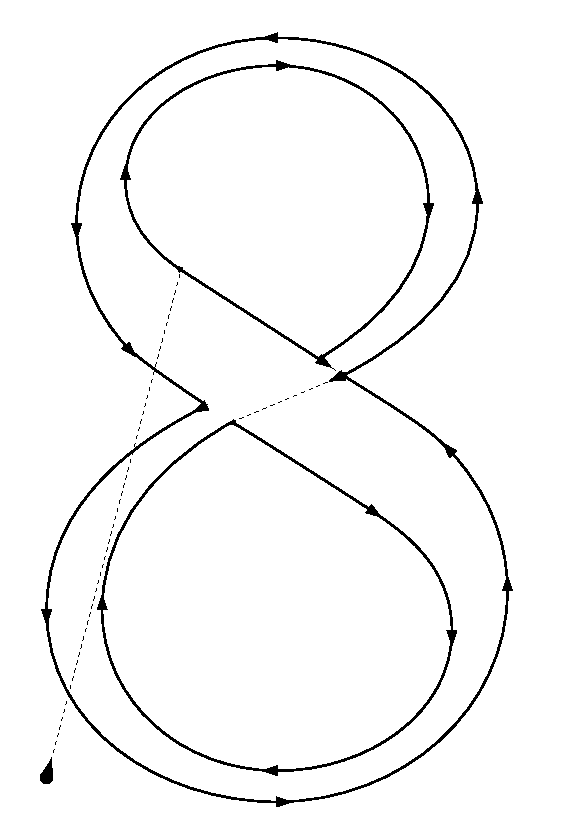
\includegraphics[scale=0.5]{t1dump/t1dump_eight}
\hfill
\fbox{B}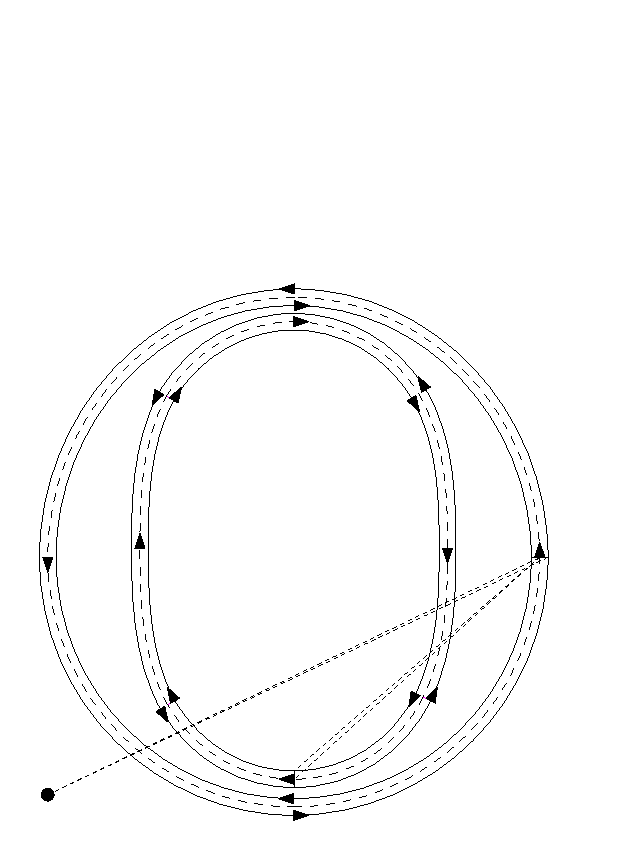
\includegraphics[scale=0.5]{t1dump/t1dump_o}
\hfill\break
\hrule\vskip3mm\small
\caption{\label{figure:stroking1}\fbox{A} Character ``8'' from font
  ComputerModern Roman. The arrows indicate the direction of the paths. From
  the outer subpath it follows that the inner region will be filled (left of the
  path). From this massive black region, the holes are cut by means of the two
  inner subpaths (and their direction). \fbox{B} The principle of creating a
  stroked character by filling a newly created set of subpaths which surround
  the original path in an appropriate manor.}
\end{figure}
We find three subpaths which by means of their direction relations yield the
filled character. 

When talking about {\em stroking}, we mean tracing a pen of finite width along
these subpaths. When doing so, a new finite (more complex) region of ink is
built. Actually we can consider this filled region being the result of filling
a newly created path that consists of two subpaths surrounding the original
path and having appropriate directions. These newly created subpaths are
referred as the {\em right path} and the {\em left path}.
Figure~\ref{figure:stroking1} \fbox{B} illustrates this idea for the
character ``o''. The original path is represented by dashed curves whereas
left paths and right paths are shown as solid curves. The respective
directions are indicated by arrows.

Now, what are the steps required to compute a right path or left path from a
given path and given a certain strokewidth? Firstly, for each path segment two
{\em parallel paths} the right and the left path, located half the strokewidth
right and left of the original path have to be computed. This is shown for the
character ``t'' in Figure~\ref{figure:stroking2}, \fbox{A}.
\begin{figure}[t]
\hfill
\fbox{A}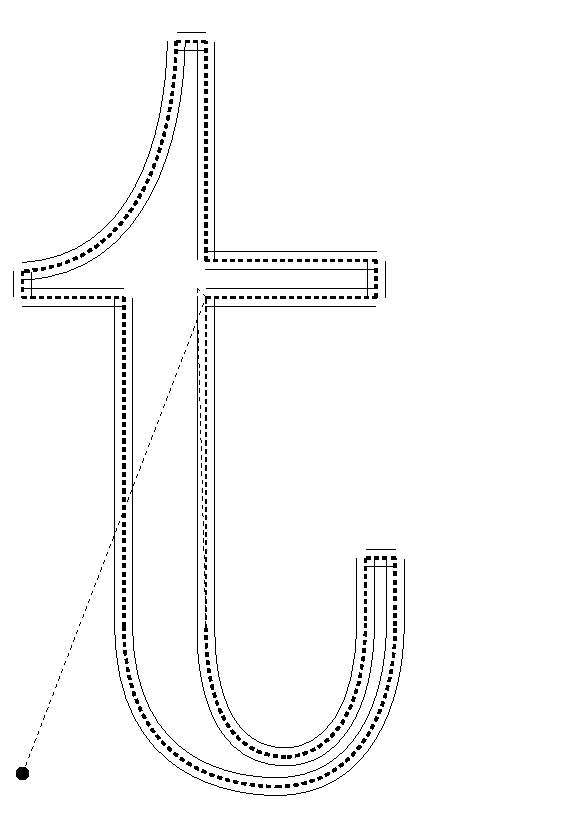
\includegraphics[scale=0.5]{t1dump/t1dump_t_1}
\hfill
\fbox{B}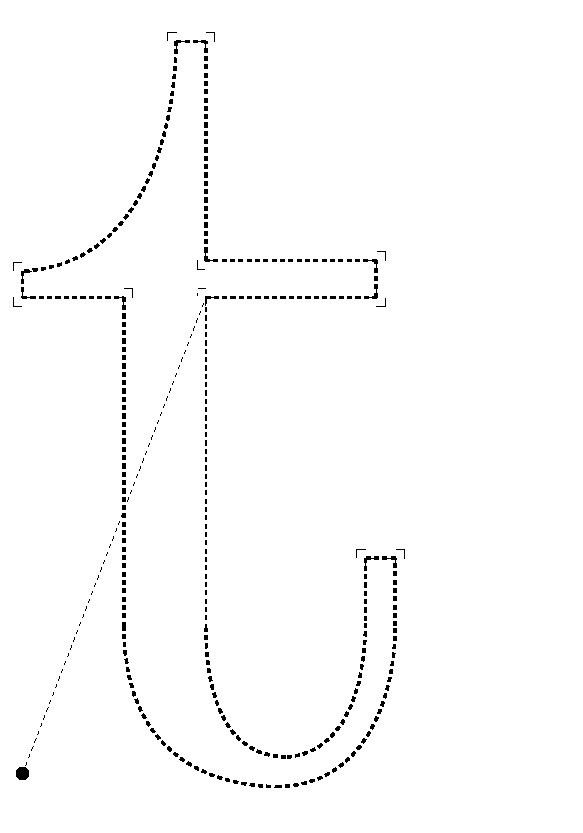
\includegraphics[scale=0.5]{t1dump/t1dump_t_2}
\hfill\break
\hrule\vskip3mm\small
\caption{\label{figure:stroking2}\fbox{A} Character ``t'' from font
  ComputerModern Roman. The original path is shown in a thick dashed
  style. Each segment is surrounded by a parallel path to the right hand side
  and a parallel path to the left hand side. 
  \fbox{B} Required additional connection segments in order to complete the
  outline path.}
\end{figure}

In particular, it turns out that in order to connect two parallel right or
left paths of two neighboring original path segments, additional path segments
are required. Therefore, in a second step, these parallel path
segments---which in general may be disjoint---have to be connected
appropriately. These additional path segments are shown in \fbox{B} of the
figure. We term these path segments {\em Prolongation Segments}. They
are always built as straight lines. It is also obvious, that for convex edges,
prolongation actually is what it indicates, and for concave edges, some trick
must be applied so that prolongation yields a path that actually {\em
  shortens} the respective parallel path segments.

\subsection{Computation of Parallel Paths}
\label{parallelpaths}%
For straight lines, the notion of a parallel path in distance $w/2$ immediately
becomes evident, but what about Bezier curves? Let us define the parallel of a
curve as the infinite set of points, that results from tracing along the
curve and for each point of the curve computing the point which in direction
orthogonally to the curve's tangent at the respective location is just the
distance $w/2$ apart.

The {\em parallel curve} resulting from the principle above actually no longer
is a third order Bezier curve. But if a few additional constraints hold, it
can be approximated quite well by such a third order Bezier curve:
\begin{itemize}
\item The curvature should not exceed an angular range of 90 degrees. This
  condition automatically is fulfilled for Type 1 fonts which adhere to the
  Adobe recommendations.
\item The strokewidth $w$ the curve should be drawn width is small compared to
  the extension and the curvature of the curve. This principle usually is
  fulfilled by nature because tracing a character outline path with a very
  thick pen won't lead to a good representation of the character.
\end{itemize}
In the following, we will describe how to compute a parallel Bezier curve
defined by four points $\vec{A}'$, $\vec{B}'$, $\vec{C}'$ and $\vec{D}'$,
given an original Bezier curve defined by four points $\vec{A}$, $\vec{B}$,
$\vec{C}$ and $\vec{D}$ and a strokewidth $w$. The computation of parallel
straight lines results as the special case of only respecting the points
$\vec{A}$ and $\vec{D}$ from these considerations. 

Figure~\ref{figure:stroking3} represents the basis of our discussion.
\begin{figure}[t]
\centerline{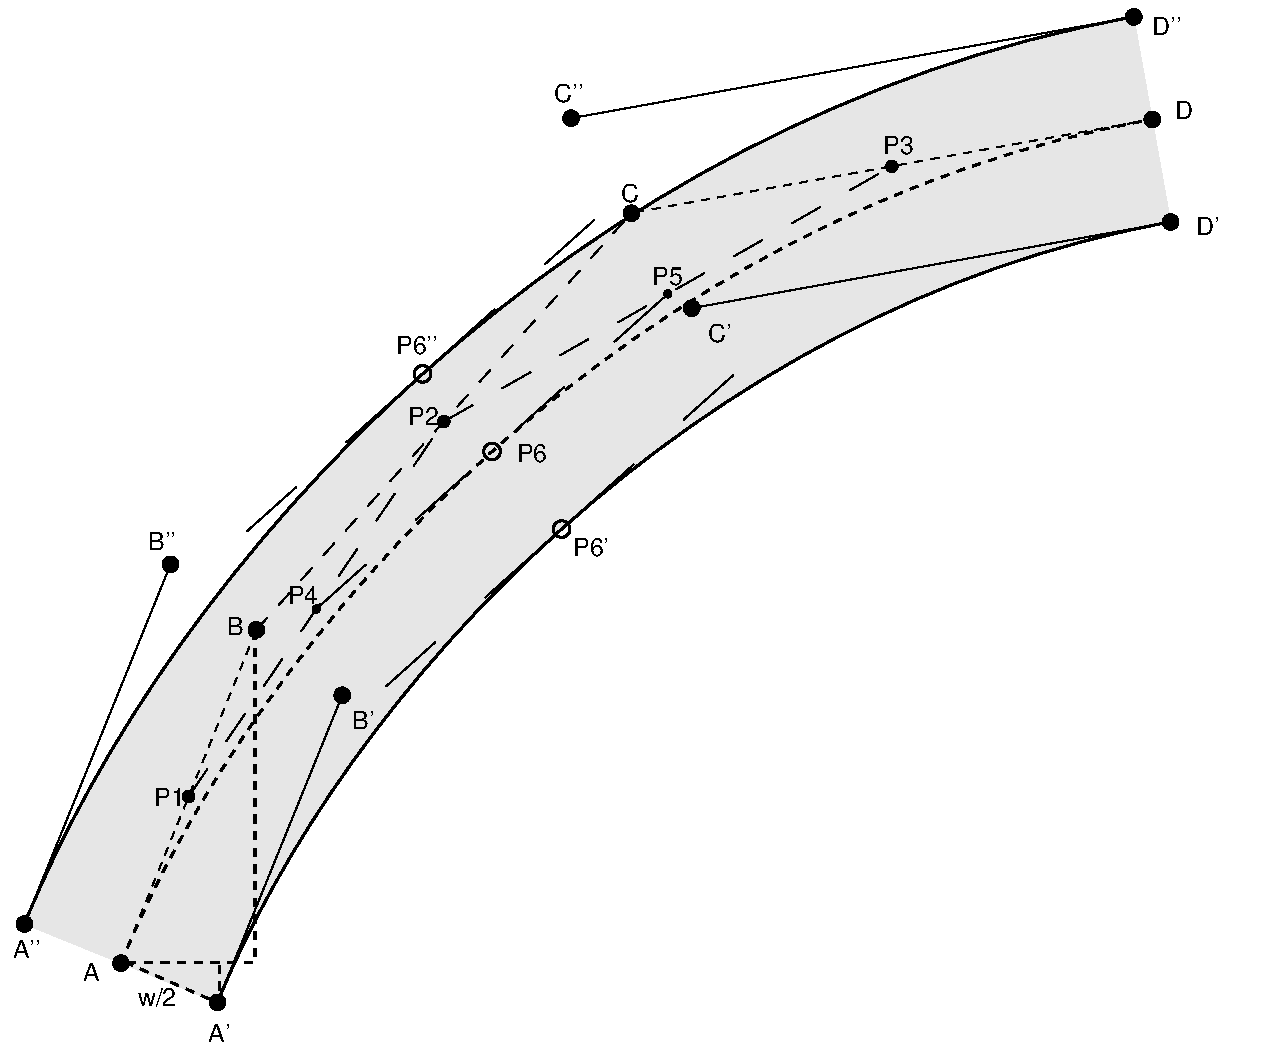
\includegraphics[scale=0.7]{t1dump/parallelpath_sk}}
\hrule\vskip3mm\small
\caption{\label{figure:stroking3}Construction of parallel Bezier path
  segments. The original curve is shown in dashed style and the light gray
  area indicates the thick Bezier curve segment that later will result from
  filling between left and right parallel path. Furthermore, important
  intermediate points are shown. A detailed discussion is given in the text.} 
\end{figure}
It shows the original mathematically thin Bezier segment defined by the points
$\vec{A}$, $\vec{B}$, $\vec{C}$ and $\vec{D}$ in dashed style. The
counterpart of $\vec{A}$ in the parallel path follows from simple geometric
considerations, as illustrated for the point $\vec{A}'$. It lies half the
strokewidth $w$ away from $\vec{A}$ and the direction is determined by the
location of point $\vec{B}$. For the two coordinates of $\vec{A}'$ we find 
\begin{equation}
  \label{eq:eq1}
  A'_x = A_x + \frac{w}{2}\frac{B_y - A_y}{|\vec{B} - \vec{A}|}
\end{equation}
and
\begin{equation}
  \label{eq:eq2}
  A'_y = A_x - \frac{w}{2}\frac{B_x - A_x}{|\vec{B} - \vec{A}|}.
\end{equation}
Corresponding equations can be derived for the point $\vec{D}'$, so that, up to now, we
are able to compute parallel straight line segments. It remains to compute two
control points, $\vec{B}'$ and $\vec{C}'$, in a way that the resulting Bezier
curve appears as parallel to the original curve in the sense defined above. 

In order to make the path at point $\vec{A}'$ actually parallel to the orginal
path at $\vec{A}$, we require $\vec{B}' - \vec{A}'$ to be parallel to $\vec{B}
- \vec{A}$. From this we can derive an equation that expresses the fact that
$\vec{B}'$ lies somewhere on the straight line that runs through point
$\vec{A}'$ and has the direction $\vec{B} - \vec{A}$, i.e.,
\begin{equation}
  \label{eq:eq3}
  \vec{B}' = \vec{A}' + \mu_B (\vec{B} - \vec{A}),
\end{equation}
and correspondingly
\begin{equation}
  \label{eq:eq4}
  \vec{C}' = \vec{D}' + \mu_C (\vec{C} - \vec{D})\phantom{,}
\end{equation}
for point $\vec{C}'$. Here, $\mu_B$ and $\mu_C$ are two positive quantities, whose
exact values are still to be determined.

In order to compute $\mu_B$ and $\mu_C$, we consider a third point on the
curve. Using a well-known algorithm that iteratively approximates a Bezier
curve via straight line segments, we can easily determine the coordinates of
the point that---in the parameter equation $f(t)$ of a Bezier
curve---corresponds to the parameter $t=1/2$. It can be considered as a {\em
  middle point} of the curve segment. In Figure~\ref{figure:stroking3}, this
point is named $\vec{P}_6$. It can be computed by computing some intermediate
points: 
\begin{equation}
  \label{eq:eq5}
  \vec{P}_1 = \frac{1}{2} ( \vec{A} + \vec{B} )
\end{equation}
\begin{equation}
  \label{eq:eq6}
  \vec{P}_2 = \frac{1}{2} ( \vec{B} + \vec{C} )
\end{equation}
\begin{equation}
  \label{eq:eq7}
  \vec{P}_3 = \frac{1}{2} ( \vec{C} + \vec{D} )
\end{equation}
\begin{equation}
  \label{eq:eq8}
  \vec{P}_4 = \frac{1}{2} ( \vec{P}_1 + \vec{P}_2 )
\end{equation}
\begin{equation}
  \label{eq:eq9}
  \vec{P}_5 = \frac{1}{2} ( \vec{P}_2 + \vec{P}_3 )
\end{equation}
and finally
\begin{equation}
  \label{eq:eq10}
  \vec{P}_6 = \frac{1}{2} ( \vec{P}_4 + \vec{P}_5 ) 
  = \frac{1}{8} ( \vec{A} + 3 \vec{B} + 3 \vec{C} + \vec{D} ) 
\end{equation}
Using the same geometrical considerations as in Eqs.~\ref{eq:eq1} and
\ref{eq:eq2}, we can now compute a unit vector, $\vec{n}_6$, perpendicular to
the curve at $\vec{P}_6$ and obtain
\begin{equation}
  \label{eq:eq11}
  n_{6x} = \frac{ P_{5y} - P_{4y} }{\sqrt{(P_{5x}-P_{4x})^2 + (P_{5y}-P_{4y})^2}}
\end{equation}
\begin{equation}
  \label{eq:eq12}
  n_{6y} = - \frac{ P_{5x} - P_{4x} }{\sqrt{(P_{5x}-P_{4x})^2 + (P_{5y}-P_{4y})^2}}
\end{equation}
$\vec{P}'_6$ can now be computed as 
\begin{equation}
  \label{eq:eq13}
  \vec{P}'_6 = \vec{P}_6 + \vec{N}_6,
\end{equation}
where $\vec{N}_6 = \frac{w}{2} \vec{n}_6$, i.e., the vector orthogonal to the
curve at $\vec{P}_6$ with a length of half the strokewidth $w$. As before, we
have to require that the slope of the curve $\vec{P}_6$ equals the one at
$\vec{P}'_6$, i.e., with respect to Figure~\ref{figure:stroking3} we find
\begin{eqnarray*}
  \vec{P}'_5 - \vec{P}'_4 & = & \nu \left( \vec{P}_5 - \vec{P}_4 \right) \\ 
  \frac{\vec{P}'_2 + \vec{P}'_3}{2} -
  \frac{\vec{P}'_1 + \vec{P}'_2}{2} 
  & = & \nu \left(
  \frac{\vec{P}_2 + \vec{P}_3}{2} -
  \frac{\vec{P}_1 + \vec{P}_2}{2} \right) \\
  \frac{\vec{C}' + \vec{D}'}{2} - 
  \frac{\vec{A}' + \vec{B}'}{2} 
  & = & \nu \left(
  \frac{\vec{C} + \vec{D}}{2} - 
  \frac{\vec{A} + \vec{B}}{2} \right)
\end{eqnarray*}
and hence finally
\begin{equation}
  \label{eq:eq14}
  \vec{C}' + \vec{D}' - \vec{A}' - \vec{B}' = \nu \left(
  \vec{C} + \vec{D} - \vec{A} - \vec{B} \right)\;.
\end{equation}
We have thus expressed the slope condition at $\vec{P}_6$ in terms of the
characteristic points of a Bezier curve and a factor, $\nu$, still to be
determined (cf.~Eqs.~\ref{eq:eq3} and \ref{eq:eq4}). On the way to
Eq.~\ref{eq:eq14}, we made use of the well-known geometrical relations
\hbox{Eqs.~\ref{eq:eq5} -- \ref{eq:eq9}}. 

Based on the same considerations that led to Eq.~\ref{eq:eq10}, we can write
the corresponding equation for the point $\vec{P}'_6$:
\begin{equation}
  \label{eq:eq15}
  \vec{P}'_6 = \frac{1}{2} ( \vec{P}'_4 + \vec{P}'_5 ) 
  = \frac{1}{8} ( \vec{A}' + 3 \vec{B}' + 3 \vec{C}' + \vec{D}' ) 
\end{equation}
Exploiting Eq.~\ref{eq:eq13} and solving for $\vec{C}'$, we can reorganize
Eq.~\ref{eq:eq15}: 
\begin{equation}
  \label{eq:eq16}
  \vec{C}' = \frac{8 (\vec{N}_6 + \vec{P}_6) - \vec{A}' - \vec{D}'}{3} -
  \vec{B}'
\end{equation}
From this equation, we are able eliminate $\vec{B}'$ by substituting the
transformed slope condition for point $\vec{P}'_6$ (Eq.~\ref{eq:eq14}). We
obtain 
\begin{eqnarray}
  \nonumber
  \vec{C}' &=& \frac{8 (\vec{N}_6 + \vec{P}_6) - \vec{A}' - \vec{D}'}{3}
  + \left[ \nu \left( \vec{C} + \vec{D} - \vec{A} - \vec{B} \right)
  - \vec{C}' - \vec{D}' + \vec{A}' \right] \\ 
  \nonumber
  2\, \vec{C}' &=& \frac{8 (\vec{N}_6 + \vec{P}_6) - \vec{A}' - \vec{D}'}{3} 
  + \vec{A}' - \vec{D}' + 
  \nu \left( \vec{C} + \vec{D} - \vec{A} - \vec{B}\right) \\
  \label{eq:eq17}
  \vec{C}' &=& 
  \underbrace{\frac{4 (\vec{N}_6 + \vec{P}_6) + \vec{A}' - 2 \vec{D}'}{3}}
  _{\mbox{$\vec{l}_C$}}
  + \frac{\nu}{2} \underbrace{\left( \vec{C} + \vec{D} - \vec{A} -
  \vec{B}\right)}
  _{\mbox{$\vec{d}_C$}} \,.
\end{eqnarray}
Here, for the sake of brevity, we introduced a location vector, $\vec{l}_C$,
and a direction vector, $\vec{d}_C$, which together with the parameter $\nu$
define the point $\vec{C}'$. 

Considering Eqs.~\ref{eq:eq4} and \ref{eq:eq17}, we finally found two
independent relations for $\vec{C}'$, that linearly depend on two quantities,
$\mu_C$ and $\frac{\nu}{2}$. Therefore, by substituting the right hand sides
of (\ref{eq:eq4}) and (\ref{eq:eq17}), we obtain the following $2 \times
2$ system of linear equations:
\begin{equation}
  \label{eq:eq18}
  \left[ 
    \begin{array}{cc}
      (\vec{C}-\vec{D}) & \vec{d}_C 
    \end{array}
  \right] 
  \left(
    \begin{array}{cc}
      \mu_C \\
      \nu/2
    \end{array}
  \right)
  = \left( \vec{l}_C - \vec{D}' \right)
\end{equation}
Formally, all vectors appearing in this equation are column vectors. The
solution of the system can be written as 
\begin{equation}
  \label{eq:eq19}
  \left(
    \begin{array}{cc}
      \mu_C \\
      \nu/2
    \end{array}
  \right)
  = 
  \left[ 
    \begin{array}{cc}
      (\vec{C}-\vec{D}) & \vec{d}_C 
    \end{array}
  \right]^{-1}
  \left( \vec{l}_C - \vec{D}' \right)\, .
\end{equation}
Once $\vec{C}'$ has been computed, it is easy to compute $\vec{B}'$, by making
use of Eq.~\ref{eq:eq16}.

A few remarks about the approach described above are appropriate.
\begin{itemize}
\item It is also possible to first compute the point $\vec{B}'$ and then use
  Eq.~\ref{eq:eq16} to compute $\vec{C}'$.
\item The numerical stability at the respective end of the curve determines
  the preference of which point to compute first. A criterion for the
  numerical stability is the absolute value of determinant of the $2 \times 2$
  matrix in Eq.~\ref{eq:eq18}.  
\item This determinant may become zero in which case the curve transforms into
  a straight line. These cases must be treated extraordinarily.
\item There are a number of further exceptional cases, e.g., if point $\vec{C}$
  equals $\vec{D}$. Then the slope at this end of the curve is not enforced by
  point $\vec{C}$.
\item A good solution, that is, a {\em parallel curve}, will only result, if
  the set of assumptions discussed previously holds. If the resulting curve
  does not appear {\em parallel} to the original curve, the parallel curve
  cannot be approximated by a third order Bezier spline.
\end{itemize}


\subsection{Connection of Path Segments and Prolongation}
\label{connectingpaths}
In order to actually obtain delimiting paths for character outlines, the
parallel paths have to be connected to a continuous path. This raises the
problem of line joining. When connecting two neighboring parallel path
segments, we have to distinguish between two qualitatively different
situations. 
\begin{enumerate}
\item Convex Corner\\
  When tracing along two neighboring parallel path segments, we turn to the
  left and a convex corner appears. In these cases, we prolongate the end of
  the first path and the beginning of the second path using straight lines and
  compute an intersection between these prolongation segments. The resulting
  lengths of both prolongation segments will be positive.
\item Concave Corner\\
  When tracing along two neighboring parallel path segments, we turn to the
  right and a concave corner results. In these cases, the two neighboring
  parallel path segments intersect by nature and actually would have to be
  trimmed to their intersection point. Trimming on the other hand would make
  it impossible to feed the resulting curve in the standard format into the
  rasterizer. We therefore use a trick that saves us computing an intersection
  and recomputing the Bezier control points. From the ideal end point of the
  first parallel path we insert a straight prolongation to the connection
  point of the original path segments and a second straight prolongation
  segment from there to the starting point of the second parallel path
  segment. Then, the area left of the path is ensured to be within the extents
  that finally are to be filled with ink. 
\end{enumerate}
We will now explain this principle using the example shown in
Figure~\ref{figure:stroking4}. 
\begin{figure}[t]
\centerline{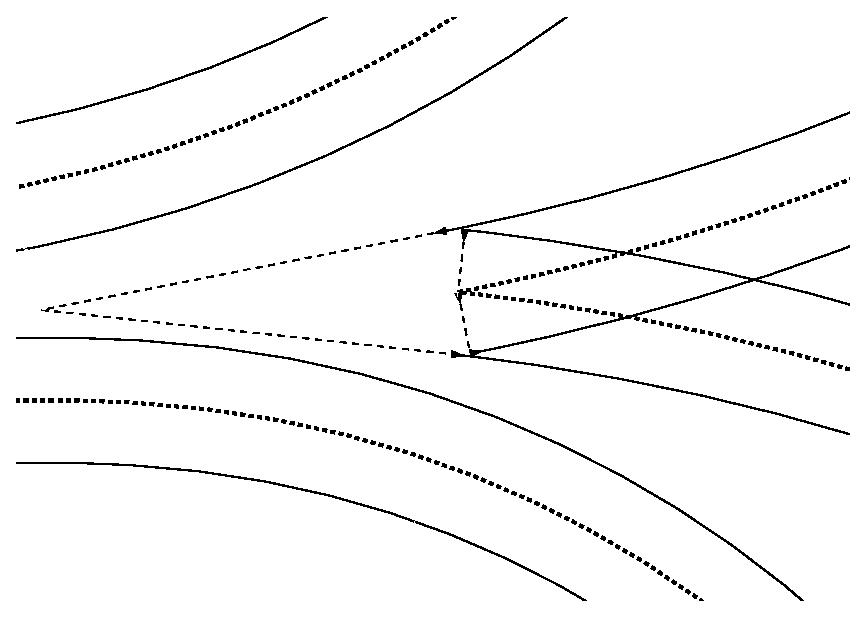
\includegraphics[scale=1.1]{t1dump/t1dump_B}}
\vskip3mm\hrule\vskip3mm\small
\caption{\label{figure:stroking4}A small excerpt at the middle right from the
  character ``B'' of ComputerModern Roman. The ideal mathematical outline of
  the filled character is shown in thick dashed style. Left and right path of
  the character's outline representation are shown in medium solid
  style. Prolongation is indicated by large dashes of medium thickness.}
\end{figure}
The interesting part is in the middle right. The original path---shown in bold
dashed style---steps into the figure in the lower right as the end of a curve
segment $p_1$. At the following connection point, the path strongly turns to
the right so that a concave corner results and continues with a further curve
segment $p_2$. This path is now to be surrounded in a symmetrical manner by
one right and one left path. For $p_1$, we find the right path as a parallel
curve segment above the original path. It has been computed as described in
the previous section. For $p_2$, the right path is a parallel curve segment
located in an appropriate distance below $p_2$. The two neighboring right path
segments are disjoint because of the concavity of the resulting corner. Hence,
rule 2 from above applies in order to connect them using straight prolongation
lines, in the figure shown in wide dashes of a medium linewidth: From the end
of right path 1, we prolongate to the point where the original segments $p_1$ and
$p_2$ join, and from there, a second prolongation to the beginning of right
path 2 is inserted. The direction is indicated by arrows. Obviously, even the
right path alone produces a closed region in this case, but this does not
cause problems here.

The left path runs into the direction opposite to the original path. By
nature, the curvature at the point under consideration now is convex. Hence,
according to rule 1, the neighboring left paths' segments are prolongated to
their common intersection point, respecting the ending direction of left
path 1 and the starting direction of left path 2.

The kind of corner at two neighboring parallel path segments $p_1$ and $p_2$
can be computed analytically. Let $\vec{T}_1$ be the tangent vector at the end
point of $p_1$ and $\vec{T}_2$ be the tangent vector at the starting point of
$p_2$. Assuming that both $\vec{T}_1$ and $\vec{T}_2$ are column vectors, we
can use the determinant of the square matrix constructed by these vectors to
determine the corner type:
\begin{equation}
  \label{eq:eq20}
  d = 
  \left| 
    \begin{array}{cc}
      \vec{T}_1 & \vec{T}_2
    \end{array}
  \right|
\end{equation}
If $d<0$, the corner type is concave whereas for $d>0$, the corner type is
convex. For the special case $d=0$, the slope at the joining point is
continuous, so that effectively $\vec{T}_1$ and $\vec{T}_2$ linearly depend on
each other. For those cases, prolongation is not required at all, because if
the neighboring segments in the original path join, neighboring segments in the
left and right path will do so too.

The kind of joining lines described above is known as {\em mitered line
  joining}. \tonelib\ does not impose a limit on the width of mitered corners,
so that the operation \tonelib\ implements is identical to what PostScript
does by default, i.e., using a line join type of 0 and an infinite miter
limit.   

%%% Local Variables: 
%%% mode: latex
%%% TeX-master: "t1lib_doc"
%%% End: 
